% =================================================================================================
% File:			gest_richieste.tex
% Description:	Defiinisce la sezione relativa ad un capitolo del documento
% Created:		2015-04-21
% Author:		Tesser Paolo
% Email:		tesser.paolo@mashup-unipd.it
% =================================================================================================
% Modification History:
% Version		Modifier Date		Change											Author
% 0.0.1 		2015-04-21 			creato scheletro doc							Tesser Paolo
% =================================================================================================
%

% CONTENUTO DEL CAPITOLO
\section{Gestione richieste recipe} % (fold)
\label{sec:gest_richieste}


	\subsection{Contenuti Sezione} % (fold)
	\label{sub:contenuti_sezione}
		L'amministratore può provvedere ad approvare o respingere l'inserimento di una nuova recipe\gloss{} proposta da un utente.\newline
		Vengono messe a disposizione dell'amministratore le seguenti funzioni:
		\begin{itemize}
			\item \textbf{See Details}: visualizza i dettagli della recipe richiesta (Figura: \ref{fig:richiesta_ricette}, rif. 1);
			\item \textbf{Discard}: disapprova la richiesta (Figura: \ref{fig:richiesta_ricette}, rif. 2);
			\item \textbf{Approve}: approva la richiesta di aggiunta (Figura: \ref{fig:richiesta_ricette}, rif. 3);
		\end{itemize}
		E' possibile visualizzare l'elenco delle recipe\gloss{} in attesa di approvazione (Figura: \ref{fig:richiesta_ricette}).
		\begin{figure}[H]
			\centering
			\centerline{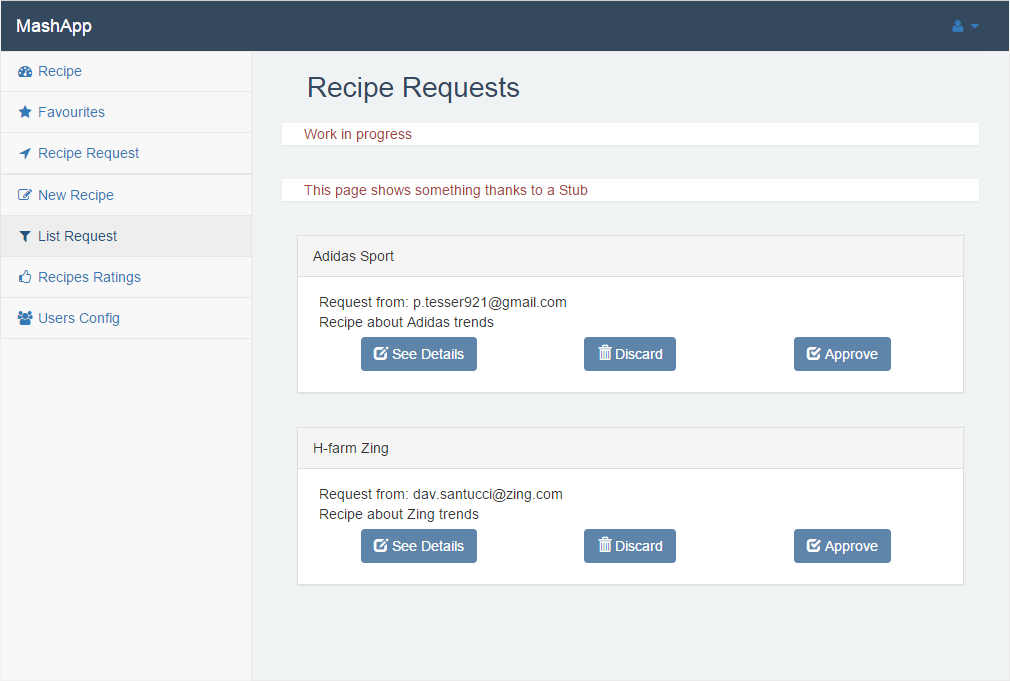
\includegraphics[width=14cm]{images/richiesta_ricette.png}}
			\caption{Approvazioni e eliminazione richieste utente}
			\label{fig:richiesta_ricette}
		\end{figure}


	\pagebreak
	\subsection{Visualizza elenco richieste}
		L'utente amministratore può visualizzare un elenco delle richieste delle recipe\gloss{} (Figura: \ref{fig:richiesta_ricette}) che sono state inviate dagli utenti normali e non ancore marcate come \textbf{chiuse}.\newline
		Per accedere all'elenco delle richieste (Figura: \ref{fig:richiesta_ricette}), selezionare l'apposito pulsante \textbf{List Request} dal menu principale della dashboard\gloss{} (Figura: \ref{fig:dashboard}).
	% END
	

	\subsection{Visualizza dettagli richiesta}
		L'utente amministratore può visualizzare tutti i dettagli di una richiesta, dopo aver premuto il pulsante \textbf{See Details} (Figura: \ref{fig:richiesta_ricette}, rif. 1) dall'elenco delle richieste.\newline
		I dettagli di una richiesta includono:
		\begin{itemize}
			\item Il nome dell'utente che l'ha inoltrata;
			\item Il titolo della richiesta;
			\item La descrizione della richiesta;
			\item L'identificativo presente sul social network.
		\end{itemize}
		Un utente amministratore può accettare o respingere una richiesta.\newline
		Può inoltre modificare il titolo o la descrizione qualora li ritenesse inopportuni.
	% END
	
	
	\subsection{Modifica richiesta Recipe}
		L'utente amministratore può modificare titolo e descrizione della richiesta per renderla più efficace da comprendere per gli altri amministratori.
		Per eseguire questa operazione occorre identificare dall'elenco delle richieste recipe\gloss{} e premere sul pulsante \textbf{See Details} (Figura: \ref{fig:richiesta_ricette}, rif. 2).
		I parametri che si possono modificare sono i seguenti:
		\begin{itemize}
		 	\item Il titolo della richiesta;
		 	\item La descrizione della richiesta;
		\end{itemize}
		Una volta terminate le modifiche è necessario selezionare il pulsante \textbf{Save} affinché queste siano attive nel sistema.
	% END

	\pagebreak
	\subsection{Accettazione richiesta}
		L'utente amministratore, una volta controllata la validità della recipe\gloss{} richiesta, potrà accettarla in modo che venga inserita nel sistema\gloss{}.\newline
		Per svolgere questa operazione occorre accedere innanzitutto all'elenco delle richieste recipe\gloss{} (Figura: \ref{fig:richiesta_ricette}) dal Menu principale della dashboard\gloss{} (Figura: \ref{fig:dashboard}).\newline
		Per confermare la richiesta basta solamente premere il pulsante \textbf{Approve} (Figura: \ref{fig:richiesta_ricette}, rif. 3) presente nell'elenco.\newline
		E' necessario confermare l'operazione selezionando il pulsante \textbf{Save} quando richiesto.\newline
		Il sistema a questo punto crea una recipe\gloss{} utilizzando i dati forniti dall'utente e confermati con l'operazione appena descritta.\newline
		Una richiesta marcata come accettata viene rimossa dall'elenco delle richieste e non più visualizzata dagli amministratori.\newline
	% END


	\subsection{Respinta richiesta}
		L'utente amministratore può decidere di rifiutare la richiesta.
		Per svolgere questa operazione è necessario accedere innanzitutto all'elenco delle richieste recipe\gloss{} (Figura: \ref{fig:richiesta_ricette}) dal Menu principale della dashboard\gloss{} (Figura: \ref{fig:dashboard}).\newline
		Per eliminare la richiesta è necessario premere il pulsante \textbf{Discard} (Figura: \ref{fig:richiesta_ricette}, rif. 2). In seguito è necessario confermare l'operazione selezionando il pulsante \textbf{Save} quando richiesto.\newline
		Una richiesta marcata come respinta viene rimossa dall'elenco delle richieste e non più visualizzata dagli altri amministratori.
	% END


% section Gestione degli utenti (end)